% latex does not allow nested imports, so include all appendices in this file as a separate 'chapter'

\appendix
\setcounter{chapter}{0}

\renewcommand{\chaptername}{Appendix}
\renewcommand{\theequation}{\Alph{chapter}.\arabic{section}.\arabic{equation}}
\setcounter{equation}{0}
\addcontentsline{toc}{chapter}{\numberline{}Appendix}

% ==========================================================================================================

\chapter{\cref{ch:study1} supplemental materials}
\label{appendix:study1}
\textit{Adapted from the online supplemental material of: }\\
Wang, H.-T., Poerio, G. L., Murphy, C. E., Bzdok, D., Jefferies, E., \& Smallwood, J. (2018). Dimensions of Experience: Exploring the Ontology of the Wandering Mind. \textit{Psychological Science}, 29 (1), 56–-71. doi: 10.1177/0956797617728727
% ==========================================================================================================
\section{Questionnaires}
\label{appendix:study1:subsection1}

\subsection{Health Organization Adult ADHD Self-Report Scale}
This is a self-report screening scale of adult ADHD, developed by the world health organisation\cite{Kessler2005}. This questionnaire comprises 18 questions to access the frequency of DSM-IV Criterion A symptoms of adult ADHD. We take the average scores across all 18 questions to access the participants’ ADHD tendency.

\subsection{Autism Spectrum Quotient}
The Autism Spectrum Quotient \cite{Baron-Cohen2001} comprises 50 questions, included 10 questions measuring 5 different dimensions: social skills, attention switching, attention to detail, communication, and imagination. For each questions the participant has four options: definitely agree, slightly agree, definitely disagree, and slightly disagree. ‘Definitely agree’ or ‘slightly agree’ responses scored 1 point on half of the designated questions.  ‘Definitely disagree’ or ‘slightly disagree’ responses scored 1 point on the other half of the questions.  The scores of each dimension is calculated with the sum of the scores of designated the questions.

\subsection{British Dyslexia Association Dyslexia checklist}
The British Dyslexia Association Dyslexia checklist \cite{Smythe2001} comprises 15 questions to access the tendency of dyslexic. Each answer of the questions have a designated scores. Individuals scoring less than 45 are probably non-dyslexic; individual scoring 45 – 60 shows a mild level of dyslexia; scoring above 60 suggests moderate or severe dyslexia. The score in the current study is the sum of the scores.

\subsection{World Health Organization Quality of Life}
The World Health Organization Quality of Life \cite{WHOQOL2002} assessment measures the quality of life cross-culturally.  In the current study, a shorter version of the original instrument, WHOQOL-BREF, was used, as it is recommended for large research studies. WHOQOL-BREF comprises 26 questions. The assessment measure the following broad domains: physical health, psychological health, social relationships, and environment. The official scoring system can be obtained on request from the official website.

\subsection{CES-Depression scale}
The CES-Depression scale \cite{Radloff1977} is a self-report scale designed to measure the symptoms of depression in the general population. The scale contains 20 questions accessing the frequency of depressive symptoms in the past one week. In the current study we used the sum of the scores as an indicator of depression.

\subsection{State-Trait Anxiety Inventory}
The State-Trait Anxiety Inventory \cite{Spielberger1987} is a measure of trait and state anxiety, composing with 20 state anxiety questions and 20 trait anxiety questions. The state anxiety questions measure the level of anxiety when taking the questionnaire; the trait anxiety questions measure the general level of anxiety. The questions are rated on a 4-point scale. Mean scores of the state and trait questions were taken as our measurement, where higher scores indicates a greater level of anxiety.

\subsection{Ruminative Response Scale}
The Ruminative Response Scale \cite{Treynor2003} is a 22-question self-report measure of rumination. Rumination involves introverted focus on negative mood and was found associating with depressive symptoms and stress \cite{Moberly2008a}. The questions are rated on a 4-point scale. Mean scores of the questions were taken as our measurement, where higher scores indicates a greater level of rumination.

% ==========================================================================================================
\section{Cognitive tasks}
\label{appendix:study1:subsection2}
The behavioural tasks were allocated into three sessions based on apparatus needed. Visual attention and generative semantic tasks were in session A, and semantic and episodic memory tasks were in session B and C. In each session, the first and second tasks were the mind-wandering task and the flanker task. In session B and C, the third task was the encoding and the delayed-recall phases of the word pair memory task respectively. The rest of the tasks were performed based on a pre-allocated order.
\subsection{General apparatus of the laboratory session}
In session B and C, the participants were in a sound proofed booth with a big glass window for the testers to monitor them. There were four testing spaces separated by office screen dividers. The tasks were delivered on Windows 7 computers and presented on 21 inches LCD monitors. Headsets were given to participants to deliver audio stimulus and blocking distracting noises. Participants were instructed to view the screen from a distance of 65 cm. The participants raised their hand to inform the experimenter to start each task. In session A, the visual attention tasks were delivered on a Windows 7 computer and presented on a 21 inches CRT monitor in a small room with light switch. The generative semantic tasks were delivered on a Windows 7 computer and presented on a 21 inches LCD monitor and a headset with microphone attached were used to recording verbal responses.
\subsection{Semantic tasks}
The tasks employed a 3 alternative force choice (3AFC) paradigm with the probe presented alongside the three choices among which the target was selected. There are four tasks: Relatedness Task (Word-to-Picture Matching; Word-to-Word Matching; Picture-to-Picture Matching), Identity Matching Task(Word-to-Picture Matching), Feature Matching Task, and Scrambled Picture Matching as the control task.

The unrelated distracters of each trial were selected among the targets from other trials ensuring that they were not linked to the probe. Except for the Feature Matching Task, all the tasks contain the same trial structure. Each trial started with 500ms blank screen. The three choices were subsequently presented on the bottom of the screen for 900ms. Finally the probe was presented on the top middle section of the screen. Probe and choices remained visible until participants’ response or for a maximum of 3 seconds. In the Feature Matching Task, the 500ms blank screen was replaced by the probe with, in bracket, the feature (cue) as criterion for the matching (colour, size, shape or texture). Probe and cue were presented for 1000ms. The three choices were subsequently presented on the bottom of the screen. Probe, cue and choices were presented as written words and remained visible until participants’ response or for a maximum of 3 seconds.

The stimuli employed in the tasks were selected from a larger dataset of words and photographs used in previous experiment
\cite{Davey2015, Krieger-Redwood2012, Krieger-Redwood2015, Whitney2012}.
The pictures were coloured photographs collected on internet and re-sized to fit the trial structure (200pixel, 72 dpi). All the coloured pictures and words were rated for familiarity and imageability using 7-point Likert scales. Lexical frequency count for the words was obtained by the SUBTLEX-UK database \cite{VanHeuven2014}.

For the details of the design, please refer to the online supplementary material of \cite{WangPsychScience2018}.

\subsection{Fluency Task}
During Verbal Fluency \cite{Adlam2010,Balota2008}, participants had 1 minute to generate as many unique words as possible belonging to a semantic category (category fluency) or starting with a specific letter (letter fluency). Semantic fluency was assessed for six categories split in two blocks (Block A: fruits, vehicles, type of dogs; Block B: animals, tools, type of boats). Letter fluency was assessed for three letter cues (Block C: A, F, S). Block order was counterbalanced across participants and the order of cues within each block was randomized. Participants’ verbal responses were collected and the audio recordings were transcribed and scored off-line.

\subsection{Word pair memory task}
Participants also undertook a Word Pair Memory Task (WPMT) to assess episodic memory \cite{Cairney2016}. 80 words were selected from an adapted version of The University of South Florida (USF) word association, rhyme, and word fragment norms \cite{Nelson2004} to create 40 semantically unrelated cue and target word pairs (e.g. owl – frame). Both the cue and target words were singular and they were matched for concreteness (t(39) = 0.39; p = .696), lexical frequency (t(39) = -4.71; p =.640), word length (t(39) = 0.09; p =.933) and number of syllables (t(39) = -0.73; p = .472). There were no pre-existing forward or backward associated relationships between any of the words, reducing the likelihood of erroneous associations between words in separate pairs.\\
During an initial learning phase, participants were presented with the unrelated words pairs, one at a time for 5 seconds each. This encoding phase was followed by a recall phase during which they attempted to recall the second word from the first word in the pair, they had 12 seconds for each trial and received a feedback after each response. In case of no response or error the feedback included the correct match. Participants were required to reach a performance criterion of 60\% correct responses, with a maximum of three repetitions of the recall phase for the entire list of word pairs. In the subsequent behavioral testing session that took place at least one day apart, participants attempted to recall the pairs immediately (without feedback) and provided a confidence rate about each of their responses using a 7-point Likert scale.

\subsection{Digit span}
For the Forward and Backward Digit Span Test we used the stimuli and the score procedure described in the WASI battery. For each trial, audio files of each digit were played in the sequential order reported in the WASI battery. The Forward and Backward Digit Span versions were tested in separate blocks and instructions were presented at the beginning of each block asking participants to listen to the sequence of numbers and type them in the same order, for the Forward block, or in reverse order for the Backward block.

\subsection{Flanker task}
We used the flanker task paradigm developed by \cite{Eriksen1974} as a baseline executive measure in this study. This task is conducted at the beginning of each laboratory sessions. The target was an arrowhead at the centre, pointing to the left or right direction. This target was flanked on either side by two to four items. The items were arrows in the same direction (congruent condition), or in the opposite direction (incongruent condition), or lines (neutral condition). The participant’s task was to identify the direction of the centrally presented arrow by pressing the left arrow key for the left direction and the right arrow key for the right direction. The stimuli were white and displayed on a black background. Each trial lasted for 4000 msec. A trial started with a fixation period of 900 - 2100 msec and then the target and the flankers appeared simultaneously. The target and the flankers were presented until the participant responded but for no longer than 1700 msec.  After the participant made a response, the target and flankers disappeared immediately and then a post-target fixation cross was presented. The duration of the post-target fixation period was based on the duration of the first fixation and RT (4000 ms minus duration of the first fixation minus RT). After this interval, the next trial began.

\subsection{Task-switching task}
\label{appendix:study1:subsection2:TS}
We used the task-switching paradigm developed by \cite{Mayr2000} and the design and task materials were constructed based on \cite{Whitmer2007}. This task measured executive control on inhibiting previously relevant information. In this task, the participant identified the spatial location of a deviant object with a verbal instruction cue. The participant used a number pad to respond. Number 1,2,4, and 5 were used. Each of them responded to the spatial location of the designated rectangle. In each trial, four blue rectangles arranged into a two-by-two matrix were displayed on screen. The rectangles can vary from each other on one of three dimensions: size, motion, or orientation. Before a set time interval of 100ms or 900ms, a verbal cue on dimensions appeared on the centre of the screen. There were one practice block and two experiment blocks. The cue-stimuli interval in the practice is 500 msec, and 900 msec and 100 msec respectively in the two experiment blocks. The trials are categorised into four: control, inhibitory, uncategorised switch and repeat, see \cite{Whitmer2007} for details.

\subsection{Four mountains task}
We used the four mountains task developed by \cite{Hartley2007} as a measure of spatial scene construction memory. In this task, the participant identified the target image that match the topography of the sample image across 30 trials. The participant was presented with a sample image of four mountains for 10 seconds, and then a four-choice of landscapes arranged in a two-by-two grid shown on the screen. The participant had no limit on thinking time for each trial, and they pressed number 1 to 4 to select the image. The target image is the same landscape as the sample image, but the perspective and environment (lighting, weather and vegetation) is changed.

\subsection{Ravens advanced progressive matrices}
The Ravens Advanced Progressive Matrices \cite<RAPM>{Raven1998} measured ‘educative ability’ – that is the ability to make sense and meaning out of complex non-verbal stimuli. In order to complete the task participants were tasked with finding new patterns and relationships between the stimuli. The RAPM used in the current study contained two tests: (i) practice test - containing 2 problems and (ii) the full test – containing 36 problems. For each problem a set of 9 boxes (ordered in a 3x3 design) were shown on the screen. All but one box contained a pattern. At the bottom of the screen were 4 additional boxes, each containing a unique pattern. Participants were required to select out of these 4 potential boxes which pattern should go in the empty box. During the practice phase participants were given online feedback outlining whether their response was correct and, if not, how they should decide which box was the correct answer. If participants had any further questions, then they were instructed to ask the experimenter before starting the main experiment. During the full test no feedback was given. Participants were given 20 minutes to complete as many problems as they could, the problems got progressively more difficult.

\subsection{Unusual uses task}
The Unusual Uses Task \cite{Guilford1967} assessed divergent thinking and creativity. Participants were instructed to list as many unusual uses as they can for a familiar object. Three objects were selected (newspaper, brick and shoe). Uses were considered ‘unusual’ if they were not the original use of the item. For example, saying ‘crosswords’ for newspaper would not be considered unusual, however saying ‘animal bedding’ would. For each object, the object name appeared on screen for two minutes and participants were required to type as many unusual uses as they could. The total number of unique uses they listed for each item was calculated. Repetition of uses was not included (e.g., saying ‘animal bedding’ and ‘bedding for animal cage’ would only count as one unusual use).  The participant’s creativity score was based upon the mean number of unusual uses across the three objects.

% ==========================================================================================================
\section{Supplementary analysis and figures}
\label{appendix:study1:subsection3}

\begin{table}[htbp]
\caption{Correlation between motion parameter (Mean FD Jenkinson) and variable of interests}
\resizebox{\textwidth}{!}{
  \begin{threeparttable}

     \begin{tabular}{r S S S S S S S S S S S}
        \toprule
         & \multicolumn{1}{c}{1-back} & \multicolumn{1}{c}{0-back} & \multicolumn{1}{c}{SEM} & \multicolumn{1}{c}{EXE} & \multicolumn{1}{c}{GEN} & \multicolumn{1}{c}{AD} & \multicolumn{1}{c}{SOC} & \multicolumn{1}{c}{DYSL} & \multicolumn{1}{c}{ATT} & \multicolumn{1}{c}{Positive/Habit} & \multicolumn{1}{c}{Spontaneous off task}\\
        \midrule
        \textit{r} & -0.140 & 0.161 & -0.186 & -0.234 & -0.046 & 0.002 & -0.007 & 0.043 & -0.007 & 0.057 & -0.096\\
        \textit{p} & 0.080 & 0.044 & 0.020 & 0.003 & 0.566 & 0.981 & 0.931 & 0.597 & 0.928 & 0.514 & 0.271\\
        \textit{N} & \multicolumn{1}{c}{157} & \multicolumn{1}{c}{157} & \multicolumn{1}{r}{157} & \multicolumn{1}{r}{157} & \multicolumn{1}{c}{157} & \multicolumn{1}{c}{157} & \multicolumn{1}{c}{157} & \multicolumn{1}{c}{157} & \multicolumn{1}{c}{157} & \multicolumn{1}{c}{134} & \multicolumn{1}{c}{134}\\
        \bottomrule
     \end{tabular}
    \begin{tablenotes}
      \item We selected participants for whom movement greater than .2mm occurred on less than 5\% of the resting state data (\textit{N} = 134) and re-ran the SCCA.

    \end{tablenotes}
  \end{threeparttable}
  \label{tab:S1}
}
\end{table}
% ==========================================================================================================

\begin{figure}[htbp]
	\centering
	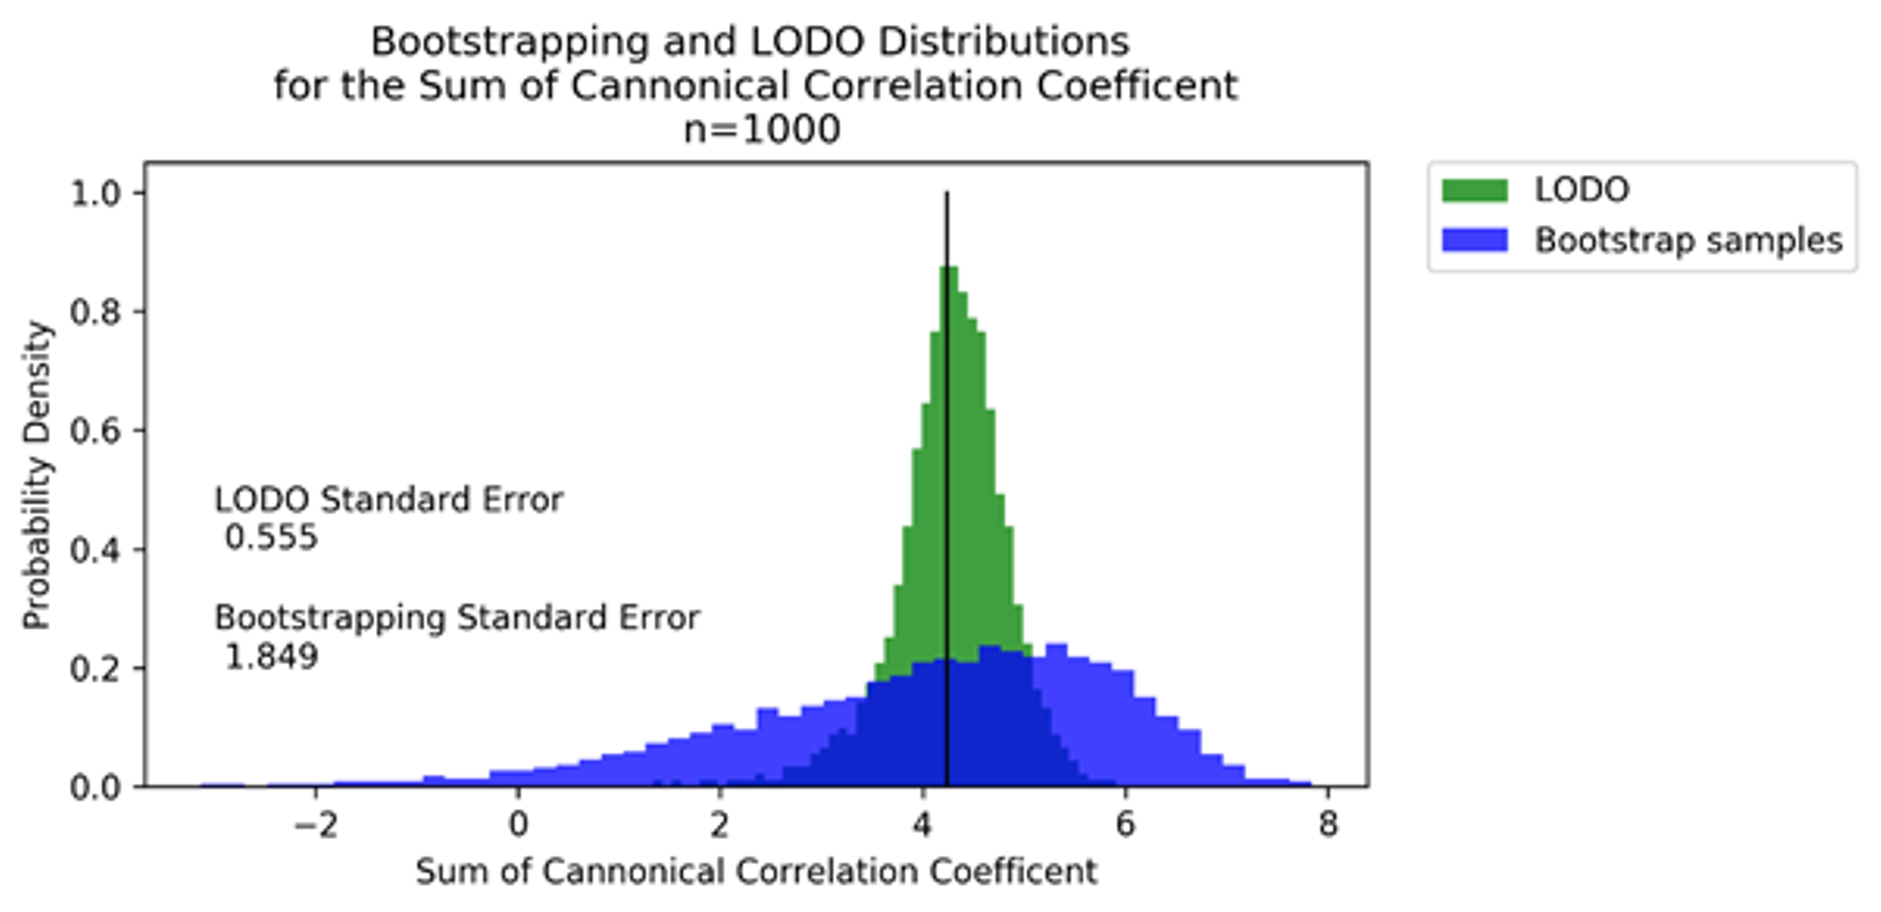
\includegraphics[width=0.8\textwidth]{append/image/study1figs1.png}
	\caption{Restricted temporal sampling and bootstrapping resampling distribution with 1000 iteration.}
	\label{fig:3S1}
\end{figure}
% ==========================================================================================================
\begin{figure}[htbp]
	\centering
	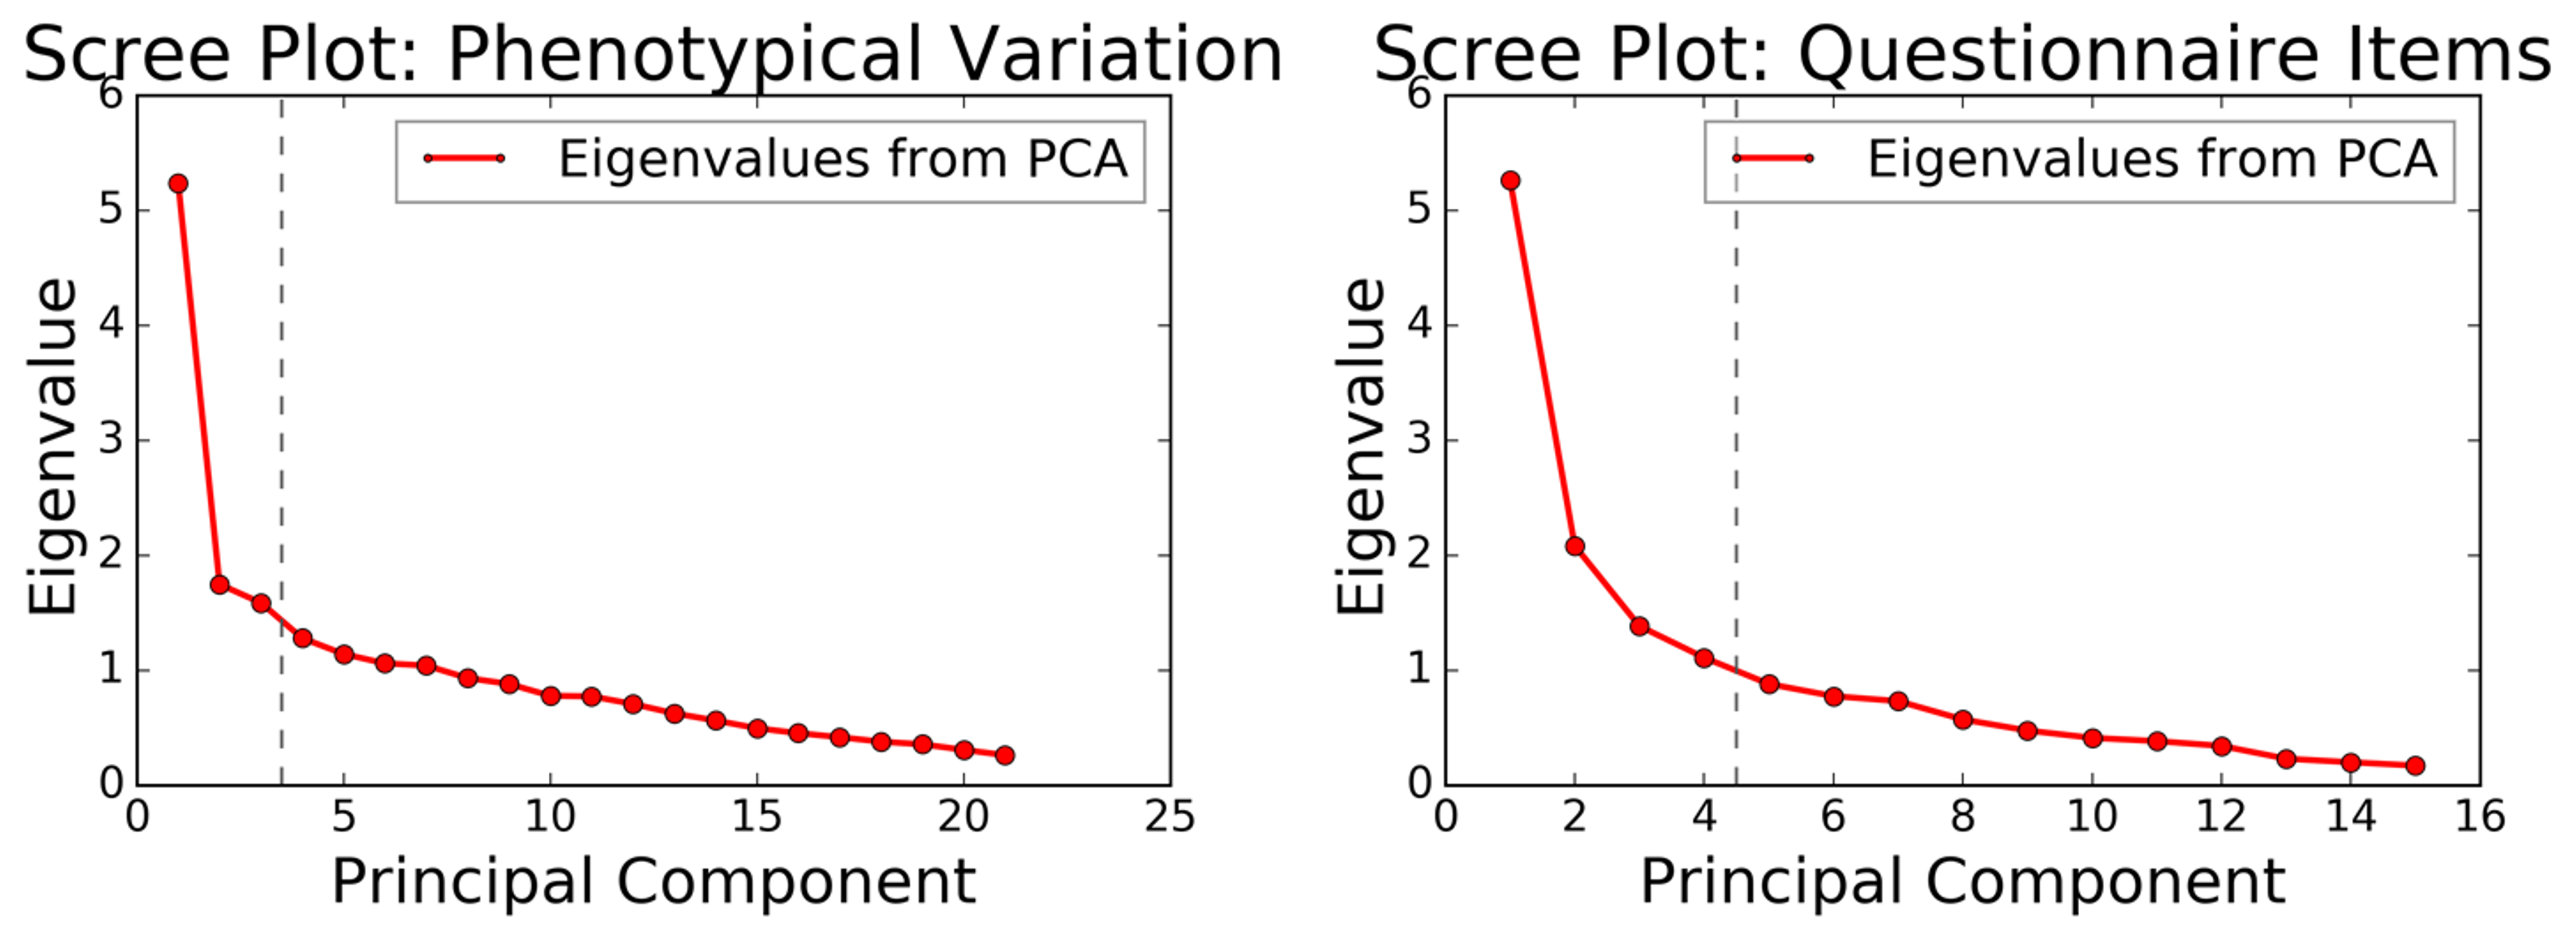
\includegraphics[width=0.8\textwidth]{append/image/study1figs2.png}
	\caption{Scree plots of the principle component analysis.}
	\label{fig:3S2}
\end{figure}
% ==========================================================================================================
\begin{figure}
    See Online Supplemental Material \url{http://journals.sagepub.com/doi/suppl/10.1177/0956797617728727}
    \caption{Full set of components.}
	\label{fig:3S3}
\end{figure}
% ==========================================================================================================
\begin{figure}
	\centering
	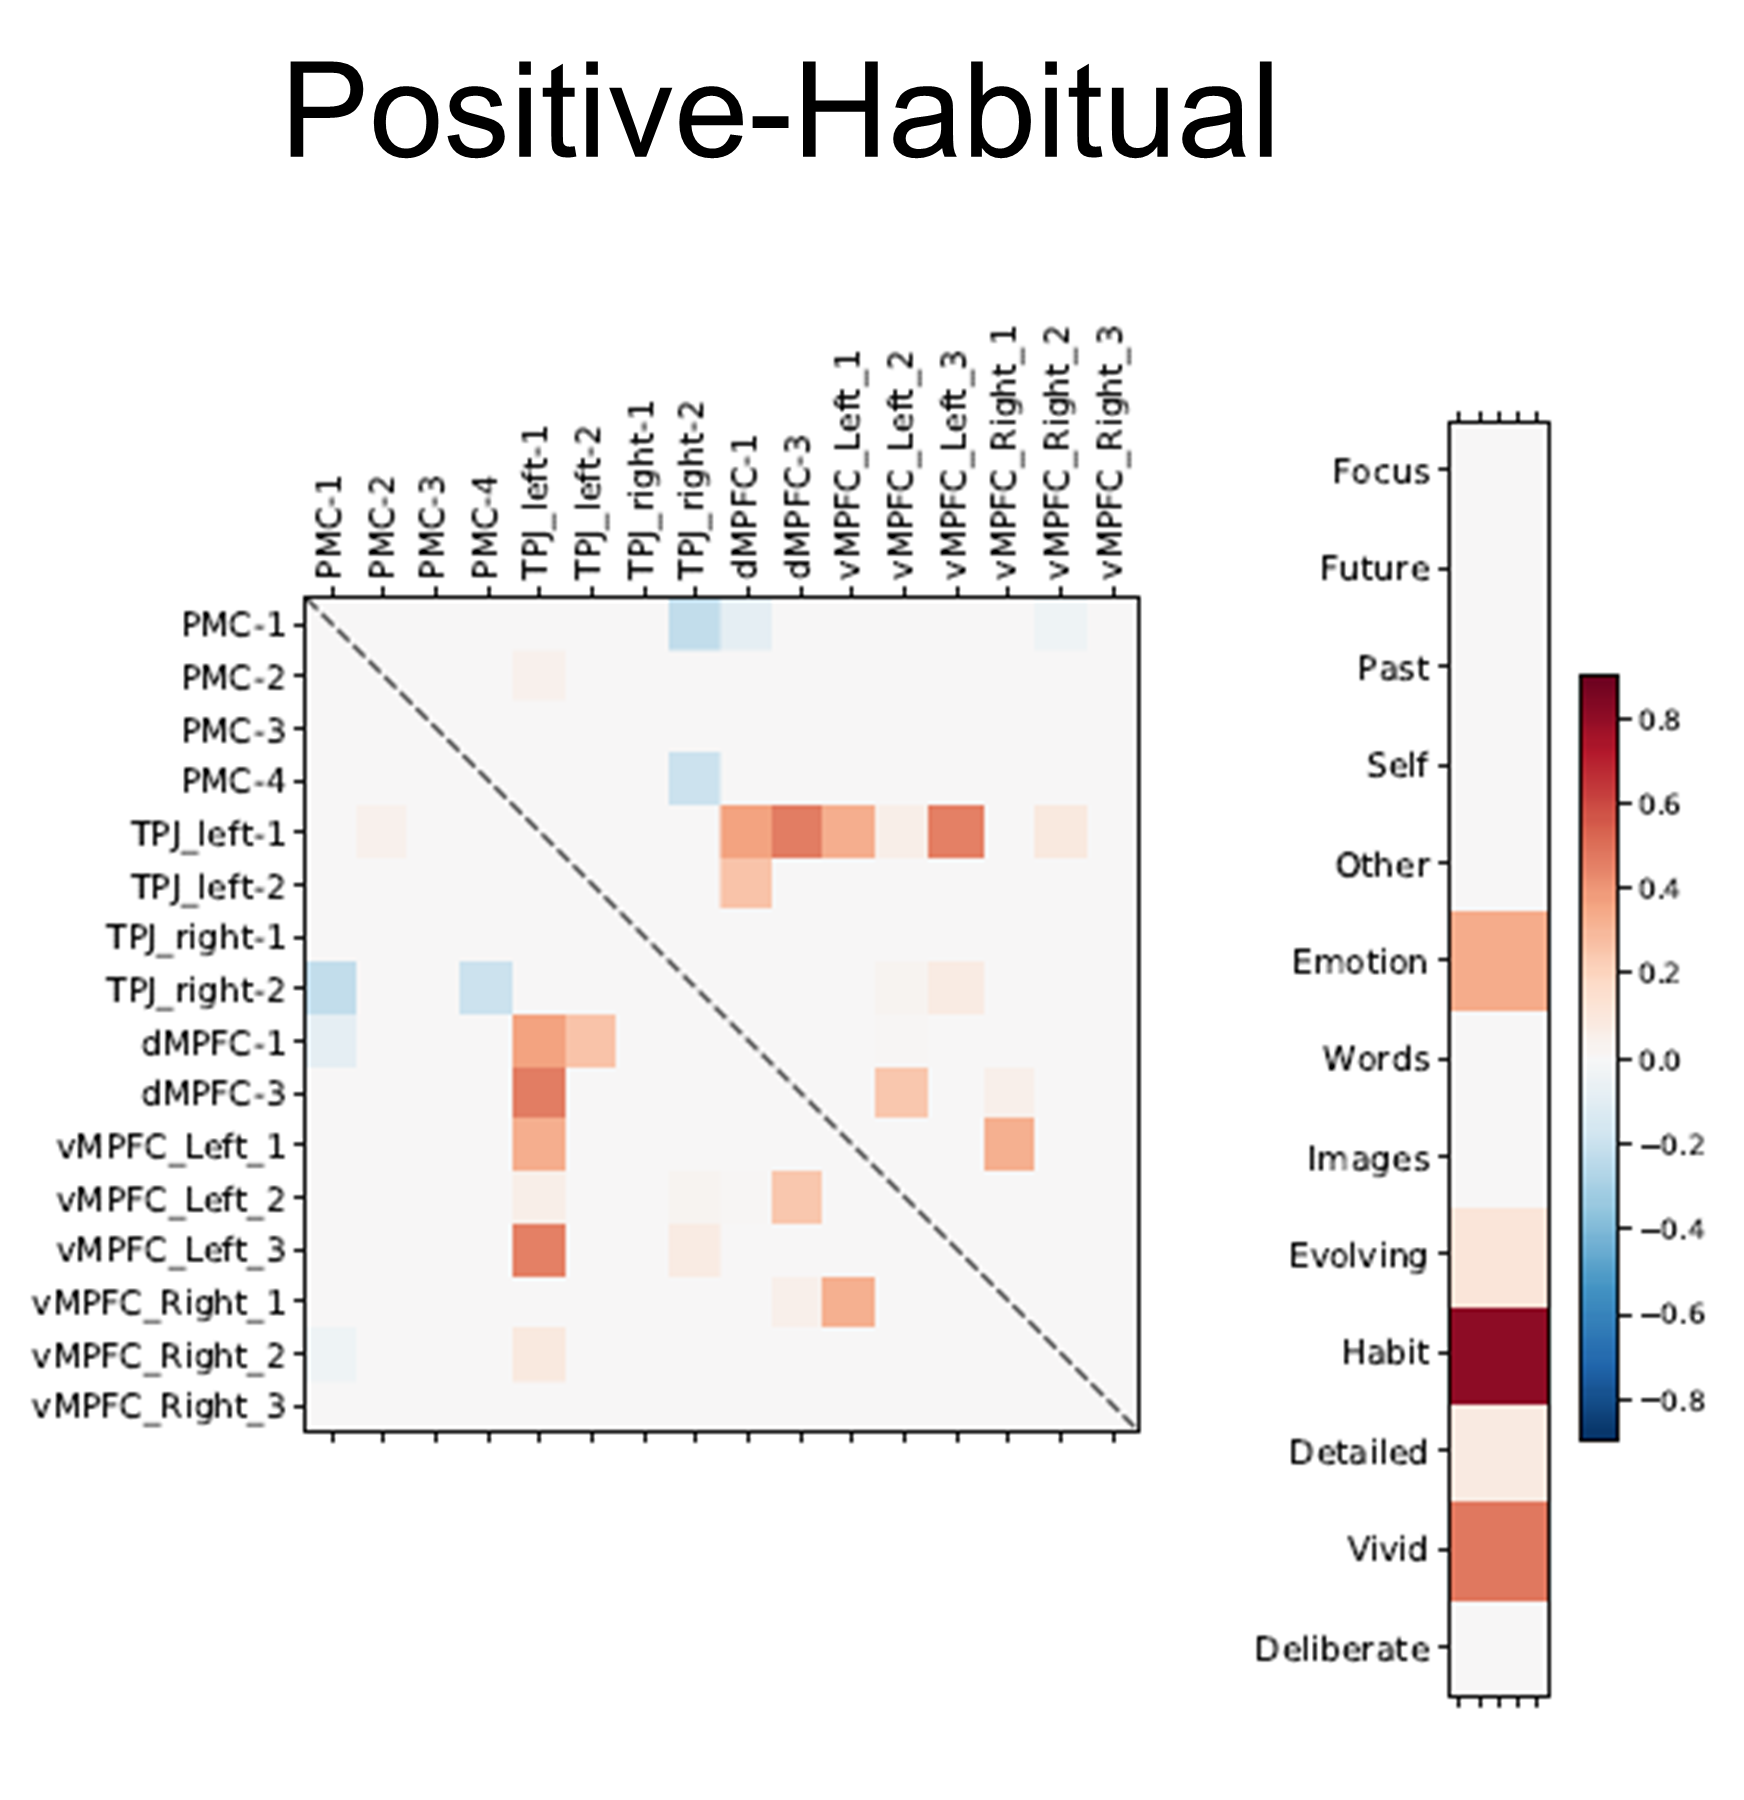
\includegraphics[width=0.6\textwidth]{append/image/study1figs4-1.png}
	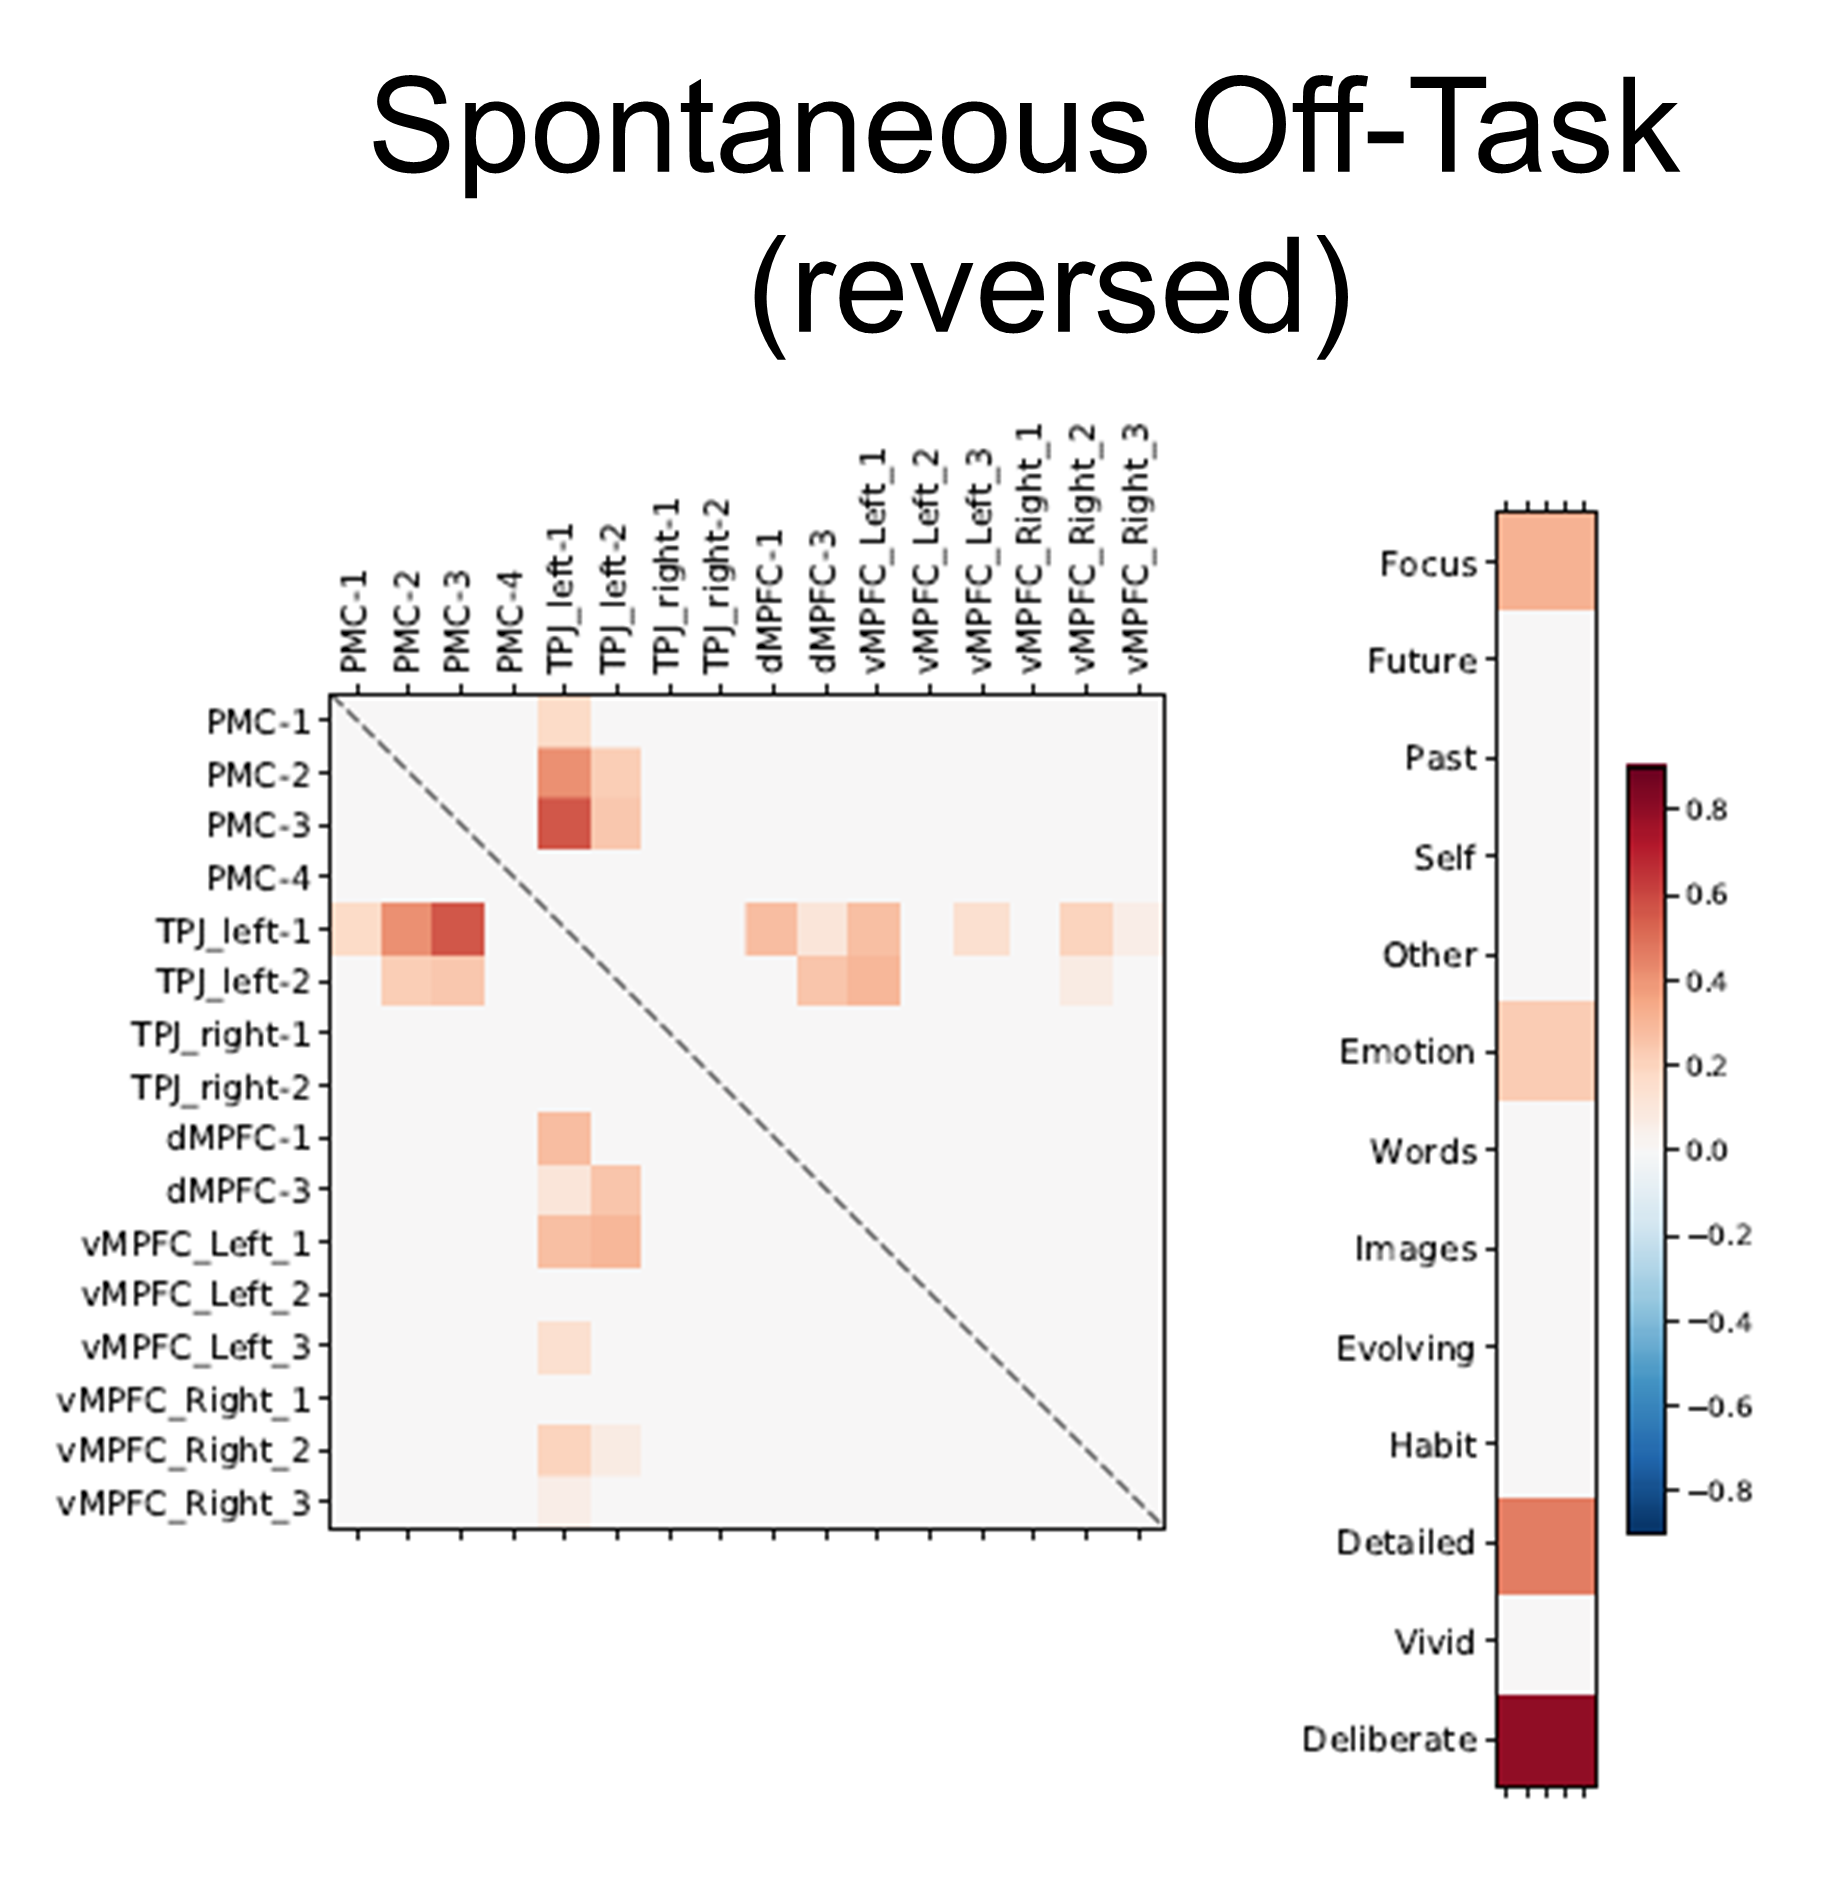
\includegraphics[width=0.6\textwidth]{append/image/study1figs4-2.png}
	\caption{Decomposition with motion outlier subjects excluded.}
	\label{fig:3S4}
\end{figure}
% ==========================================================================================================
\chapter{Nested k-fold cross-validation}
\label{appendix:kfold}

\linespacesmall
\begin{algorithm}[htb]\footnotesize
\begin{algorithmic}[1]
\parbox{15.0cm}
{
\FOR{\textit{Each outer fold k}}
    \FOR{\textit{Each parameter set}}
        \STATE Separate the development set into j folds.
        \FOR{\textit{Each inner fold j}}
                \STATE Train the model on the training set
                \STATE Calculate test error in the validation set j
        \ENDFOR
        \STATE Compute the average inner cross-validation test error
    \ENDFOR

    \STATE Choose the best parameter set with minimum average test error.
    \STATE Use this parameter set to train on the development set.
    \STATE Calculate test error in the test set
\ENDFOR
\STATE Determine the optimal model based on the outer fold test error
\STATE Train the full dataset on the optimal model
}
\end{algorithmic}
\caption{: Nested k-fold cross-validation}
\label{algorithm:1}
\end{algorithm}
\linespacenormal

% ==========================================================================================================


